\documentclass[]{article}
\usepackage[margin=2cm]{geometry}

%opening
\title{Exercises Set: Constrained Optimization}
\author{DSBA Mathematics Refresher 2026}
\date{}

\usepackage{amsmath}
\usepackage{amsfonts}
\usepackage{amsthm}
\usepackage{amssymb}
\usepackage{mathrsfs}
\usepackage{stmaryrd}
\usepackage{tikz}
\usepackage{graphicx}

\newcommand{\Q}{\mathbb{Q}}
\newcommand{\N}{\mathbb{N}}
\newcommand{\Z}{\mathbb{Z}}
\newcommand{\R}{\mathbb{R}}
\newcommand{\Primes}{\mathbb{P}}
\newcommand{\st}{\text{ s.t. }}
\newcommand{\txtand}{\text{ and }}
\newcommand{\txtor}{\text{ or }}
\newcommand{\lxor}{\veebar}
\newcommand{\vecx}{ \vec{\mathbf{x}} }
\newcommand{\vecxk}{ \vec{\mathbf{x_k}} }
\newcommand{\vecw}{ \vec{\mathbf{w}} }



\begin{document}

	\maketitle

	\begin{abstract}
		Only the questions with a * are compulsory (but do all of them!).
	\end{abstract}

	\section{Lagrangian multiplier technique}
	\begin{center}
		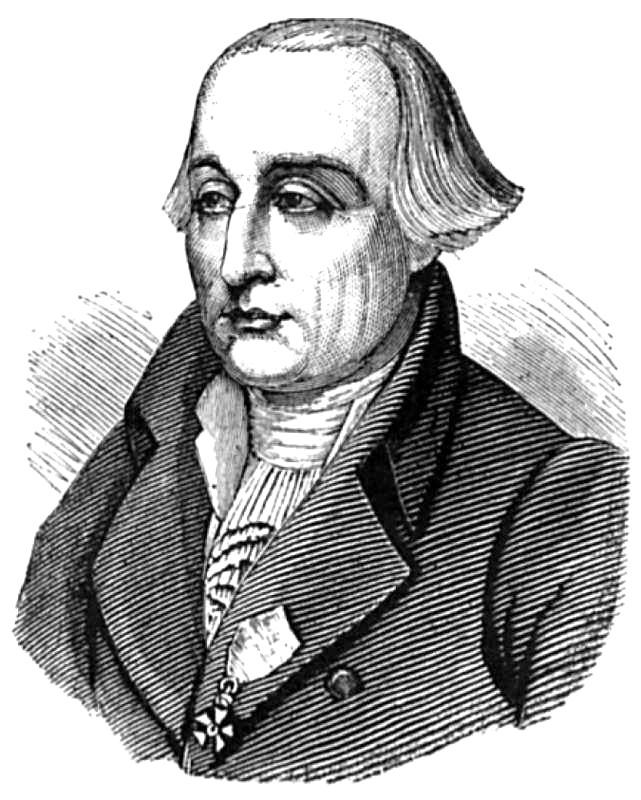
\includegraphics[height=4cm]{Lagrange}
	\end{center}
	
	\subsection{Unconstrained optimization}
	Let $f(x,y) = 2x^2-12x + 4y^2 + 8y + 20$.\\
	Find $(x^*,y^*) \in \R^2$ such that $f$ reaches its minimum (i.e. $f(x^*,y^*) \leq f(x,y) \quad \forall (x,y) \in \R^2$).
	
	\subsection{(Equality) Constrained optimization}
	Let $f(x,y) = 2x^2-12x + 4y^2 + 8y + 20$.\\
	Suppose further that we want $3x + 5y = 2$.\\
	Find $(x^*,y^*) \in \R^2$ such that $3x^* + 5y^* = 2$ and $f$ reaches its minimum (i.e. $f(x^*,y^*) \leq f(x,y) \quad \forall (x,y) \in \R^2,\ 3x + 5y = 2$).
	
	\subsection{Lagrange multiplier (*)}
	Let $f(x,y) = 2x^2-12x + 4y^2 + 8y + 20$.\\
	Suppose further that we want $3x + 5y = 2$.\\
	Let $\mathcal{L}(x,y,\lambda) = f(x,y) - \lambda (3x +5y - 2)$.\\
	Find the point where $\nabla \cdot \mathcal{L} = 0$
	
	\subsection{(Inequality) Constrained optimization}
	Let $f(x) = x^2-2x$.\\
	Suppose further that we want $3x \leq 2$.\\
	Find $x^* \in \R$ such that $3x^* \leq 2$ and $f$ reaches its minimum (i.e. $f(x^*) \leq f(x) \quad \forall x \in \R,\ 3x \leq 2$).
	\vspace{0.5cm}
	\\
	Let $f(x) = x^2+2x$.\\
	Suppose further that we want $3x \leq 2$.\\
	Find $x^* \in \R$ such that $3x^* \leq 2$ and $f$ reaches its minimum (i.e. $f(x^*) \leq f(x) \quad \forall x \in \R,\ 3x \leq 2$).
	
	\subsection{Lagrange multiplier (*)}
	Let $f(x) = x^2-2x$.\\
	Suppose further that we want $3x \leq 2$.\\
	Let $\mathcal{L}(x,\lambda) = f(x) - \lambda (-3x + 2 - s^2)$.\\
	Find the point where $\nabla \cdot \mathcal{L} = 0$ and $\lambda \geq 0$.
	\vspace{0.5cm}
	\\
	Let $f(x) = x^2+2x$.\\
	Suppose further that we want $3x \leq 2$.\\
	Let $\mathcal{L}(x,\lambda) = f(x) - \lambda (-3x + 2 - s^2)$.\\
	Find the point where $\nabla \cdot \mathcal{L} = 0$ and $\lambda \geq 0$.

	\vspace{0.5cm}

	Compare the two cases above.
	In one of them the constraint "did nothing", in the other it "pushed" the solution away from the unconstrained minimum.\\
	In which case did you find $\lambda = 0$?
	Can you explain why?


	\subsection{Distance from a point to a line}
	Let $f(x,y) = x^2 + y^2$.\\
	Suppose further that we want $2x + y = 5$.\\
	Solve this problem three times, with three different methods:
	\begin{enumerate}
		\item \textbf{Geometrically:} $f(x,y)$ is the squared distance from $(x,y)$ to the origin, so the problem asks for the point of the line $2x+y=5$ that is closest to the origin.
		Draw the line, and find that point using a geometric argument.
		\item \textbf{By substitution:} express $y$ in terms of $x$ using the constraint, substitute it in $f$, and minimize the resulting function of a single variable.
		\item \textbf{With a Lagrange multiplier:} let $\mathcal{L}(x,y,\lambda) = f(x,y) - \lambda(2x + y - 5)$, and find the point where $\nabla \mathcal{L} = 0$.
	\end{enumerate}
	Check that the three methods give the same answer.

	\subsection{A constraint that cannot be substituted}
	Let $f(x,y) = x + y$.\\
	Suppose further that we want $x^2 + y^2 = 1$ (i.e. the point $(x,y)$ is on the unit circle).

	\begin{enumerate}
		\item Try the substitution method: solve the constraint for $y$.
		What goes wrong?
		\item Use a Lagrange multiplier instead: let $\mathcal{L}(x,y,\lambda) = f(x,y) - \lambda(x^2 + y^2 - 1)$, and find all the points where $\nabla \mathcal{L} = 0$.
		\item You should find two points.
		One is the minimum of $f$ on the circle, the other is the maximum.
		Which is which?
		\item Draw the circle, and draw a few level lines of $f$ (i.e. the lines $x + y = c$ for several values of $c$).
		What is special about the level line passing through the two points you found?
	\end{enumerate}
	\begin{center}
		\begin{tikzpicture}[scale=1.55]
			\draw[->] (-1.6,0) -- (1.75,0) node[right] {\scriptsize $x$};
			\draw[->] (0,-1.6) -- (0,1.75) node[above] {\scriptsize $y$};
			\draw[thick] (0,0) circle (1);
			\draw (1,0.04) -- (1,-0.04); \node[below right] at (1,-0.02) {\scriptsize $1$};
			\draw (0.04,1) -- (-0.04,1); \node[above left] at (-0.02,1) {\scriptsize $1$};
			\node[right] at (0.78,-0.85) {\scriptsize $x^2+y^2=1$};
			\draw[gray] (0.78,-0.82) -- (0.6,-0.8);
		\end{tikzpicture}
	\end{center}
	\textit{This last question is the whole idea behind the method: at the optimum, the level line of $f$ is tangent to the constraint, which is exactly what $\nabla f = \lambda \nabla g$ says.}

	\subsection{Several constraints}
	Let $f(x,y,z) = x^2 + y^2 + z^2$.\\
	Suppose further that we want both $x + y + z = 6$ and $x - y = 2$.\\
	When there are several constraints, we use one multiplier per constraint:
	$$\mathcal{L}(x,y,z,\lambda,\mu) = f(x,y,z) - \lambda(x + y + z - 6) - \mu(x - y - 2)$$
	Find the point where $\nabla \mathcal{L} = 0$, and give the minimum value of $f$.

	\subsection{Interpreting $\lambda$: the shadow price}
	A company produces two goods, in quantities $x \geq 0$ and $y \geq 0$.
	Producing them costs $2$ per unit of $x$ and $3$ per unit of $y$, and the budget is $12$:
	$$2x + 3y = 12$$
	The utility of the production is $U(x,y) = xy$, which we want to maximize.

	\begin{enumerate}
		\item Let $\mathcal{L}(x,y,\lambda) = U(x,y) - \lambda(2x + 3y - 12)$, and find the point where $\nabla \mathcal{L} = 0$.
		Give the optimal quantities $(x^*, y^*)$, the value of $\lambda$, and the utility $U(x^*,y^*)$.
		\item Redo the computation with a budget of $B$ instead of $12$ (keep $B$ as a letter).
		Show that the optimal utility is $U^*(B) = \frac{B^2}{24}$.
		\item Compute $\frac{d U^*}{d B}$ at $B = 12$, and compare it with the $\lambda$ you found in question 1.
	\end{enumerate}
	\textit{The multiplier $\lambda$ is not just a computational trick: it measures how much the optimum improves when the constraint is relaxed by one unit.
	Economists call it the "shadow price" of the constraint.}

	\subsection{Inequality constraints in two dimensions}
	Let $f(x,y) = (x-3)^2 + (y-2)^2$.

	\begin{enumerate}
		\item First, find the unconstrained minimum of $f$ (no computation needed if you recognise what $f$ measures).
		\item Suppose now that we want $x + y \leq 6$.
		Is the unconstrained minimum still allowed?
		What is the solution of the constrained problem?
		\item Suppose instead that we want $x + y \leq 4$.
		Is the unconstrained minimum still allowed?
		Find the solution, using a drawing to guide you.
		\item Redo question 3 with a Lagrange multiplier and a slack variable:
		write the constraint as $4 - x - y \geq 0$, let
		$$\mathcal{L}(x,y,s,\lambda) = f(x,y) - \lambda(4 - x - y - s^2)$$
		and find the points where $\nabla \mathcal{L} = 0$ and $\lambda \geq 0$.
		Remember to discuss the two cases $\lambda = 0$ and $s = 0$ separately.
		\item In question 2 and in question 3, what is the value of $\lambda$?
		What does $\lambda = 0$ tell you about the constraint?
	\end{enumerate}

	\subsection{Towards Principal Component Analysis}
	Let $f(x,y) = 3x^2 + 2xy + 3y^2$.\\
	Suppose further that we want $x^2 + y^2 = 1$.

	\begin{enumerate}
		\item Let $\mathcal{L}(x,y,\lambda) = f(x,y) - \lambda(x^2 + y^2 - 1)$, and write the two equations $\frac{\partial \mathcal{L}}{\partial x} = 0$ and $\frac{\partial \mathcal{L}}{\partial y} = 0$.
		\item Show that these two equations can be written as
		$$A \begin{pmatrix} x \\ y \end{pmatrix} = \lambda \begin{pmatrix} x \\ y \end{pmatrix}
		\qquad \text{with} \qquad
		A = \begin{pmatrix} 3 & 1 \\ 1 & 3 \end{pmatrix}$$
		In other words: the possible values of $\lambda$ are the \textbf{eigenvalues} of $A$, and the candidate points are its \textbf{eigenvectors}!
		\item Find the eigenvalues and eigenvectors of $A$, and deduce the two candidate points on the unit circle (do not forget to normalize them, since we need $x^2+y^2=1$).
		\item Compute $f$ at each candidate point.
		What do you notice when you compare these values with the eigenvalues?
		\item Conclude: which direction maximizes $f$ on the unit circle?
	\end{enumerate}
	\textit{This is exactly the computation behind Principal Component Analysis: the first principal component is the unit vector maximizing a quadratic form, and it turns out to be the eigenvector associated with the largest eigenvalue.}





\end{document}
